% !TEX root = Final_Report.tex

\section{Finite-Temperature Study}
\label{sec:finite_temperature}

As a first step towards constructing the temperature-field phase diagram, it is useful to gain some familiarity with the mean-field equations at finite temperature by investigating the Kondo model in the absence of a magnetic field. The isotropy of this zero-field case will allow for convenient simplification of some terms in the mean-field equations.

\subsection{Obtaining the Mean-Field Equations}
\label{subsec:obtaining_MF}

We start by deriving the self-consistency equations that must hold for the mean-field description of the system. Since $ F = - T \ln{Z} $, searching for the minimal action is equivalent to directly minimising of $ F $, illustrating a correspondence between the path integral and a more traditional way of approaching mean-field theory. Having introduced new bosonic fields to the Lagrangian of Eq~\eqref{eq:Lagrangian}, all fermionic fields may be integrated out as outlined in Appendix~\ref{sec:Free_Energy} to obtain an effective free energy
\begin{align}
\begin{split}
F \quad = \quad & \overbrace{- 2 T~\Re~{\sum_{\sigma}\ln{\left[\frac{\widetilde{\Gamma}(\xi_{\sigma} + D)}{\widetilde{\Gamma}(\xi_{\sigma})} \right]}}}^{F_0} + \frac{2 \Delta}{\pi \rho J} - \sum_{\sigma} \lambda_{\sigma} (p_{\sigma}^2 + d^2)\\
&+ \lambda_{\text{KR}} (e^2 + \sum_{\sigma} p_{\sigma}^2 + d^2 - 1) + \lambda_{\text{SC}} (e^2 + d^2) \underbrace{- T \ln{\left( 1 + e^{\beta K \lambda_{\text{SC}}} \right)}}_{F_{\text{h}}}
\label{eq:Free_Energy}
\end{split}
\end{align}

in terms of the \textit{gamma function} $ \widetilde{\Gamma} (z) \equiv \Gamma (\frac{1}{2} + \frac{z}{2 \pi i T}) $ and $ \xi_{\sigma} = \lambda_{\sigma} + i z_{\sigma}^2 \Delta $, a complex resonance-level energy made slightly different by the inclusion of the KR term. The intermediate summation that gives rise to $ F_0 $ has been regulated by a cut-off $ D $, the half-bandwidth, to reflect the fact that electrons of arbitrarily high energies do not exist within a metal.

% Give an explanation of terms

Note that the temperature dependence of this free energy is solely contained in $ F_0 $ and $ F_{\text{h}} $, which are the only terms that differ from the existing preliminary zero-temperature study of the soft-constraint approach. We now minimise this free energy to obtain a set of mean-field equations generalised to finite temperature, starting with the Hubbard-Stratonovich field

\begin{equation}
\frac{\partial F}{\partial \Delta} = 0 \implies \sum_{\sigma} \left[ \frac{\partial F_{0}}{\partial \xi_{\sigma}} - \frac{\partial F_{0}}{\partial \overline{\xi_{\sigma}}} \right] i z^2_{\sigma} = - \frac{2}{\pi J \rho} ~ .
\label{eq:MF_delta}
\end{equation}

Though strictly free to only treat bosonic variables as complex numbers, we also restrict our search to real solutions, leading to one equation for each KR boson\footnote{This may be partly justified by the phase invariance of most terms apart from $ z_{\sigma}^2 $, which is also why we have dropped modulus-squared signs for the KR bosons throughout.}: % Give more information in the footnote about how giving different phases to e d p could mess things up

\begin{align}
\frac{\partial F}{\partial d} = 0 &\implies \sum_{\sigma} \left[ \frac{\partial F_{0}}{\partial \xi_{\sigma}} - \frac{\partial F_{0}}{\partial \overline{\xi_{\sigma}}} \right] \frac{\partial z^2_{\sigma}}{\partial d} ~ i \Delta = -d ~ ( \lambda_{\text{KR}} + \lambda_{\text{SC}} -  \sum_{\sigma} \lambda_{\sigma} ) ~ , \label{eq:MF_d} \\
\frac{\partial F}{\partial e} = 0 &\implies \sum_{\sigma} \left[ \frac{\partial F_{0}}{\partial \xi_{\sigma}} - \frac{\partial F_{0}}{\partial \overline{\xi_{\sigma}}} \right] \frac{\partial z^2_{\sigma}}{\partial e} ~ i \Delta = -e ~ ( \lambda_{\text{KR}} + \lambda_{\text{SC}} ) ~ , \label{eq:MF_e} \\
\frac{\partial F}{\partial p_{\sigma}} = 0 &\implies \sum_{s} \left[ \frac{\partial F_{0}}{\partial \xi_{s}} - \frac{\partial F_{0}}{\partial \overline{\xi_{s}}} \right] \frac{\partial z^2_{s}}{\partial p_{\sigma}} ~ i \Delta = - p_{\sigma} ~ (\lambda_{\text{KR}} - \lambda_{\sigma}) ~ . \label{eq:MF_p}
\end{align}

The form of the $ \partial z^2_{\sigma} $ derivative terms are irrelevant for the time being, but are found in Appendix~\ref{sec:MF_eq_details}. Use of the chain rule means that the difficult derivative term
\begin{equation}
\frac{\partial F_{0}}{\partial \xi_{\sigma}} - \frac{\partial F_{0}}{\partial \overline{\xi_{\sigma}}} = \frac{i}{\pi} \Re{( \widetilde{\psi}(\xi_{\sigma} + D) - \widetilde{\psi}(\xi_{\sigma}))}
\label{eq:real_derivative}
\end{equation}
appears repeatedly, where $ \psi(z) \equiv \frac{d}{\,dz}(\ln{\Gamma(z)}) $ defines the \textit{digamma function}.

% Change all the - \sigma to a \overline{\sigma}

Finally, imposing Lagrange multiplier constraints completes the set of mean-field equations:
\begin{align}
\frac{\partial F}{\partial \lambda_{\sigma}} = 0 &\implies \left[ \frac{\partial F_{0}}{\partial \xi_{\sigma}} + \frac{\partial F_{0}}{\partial \overline{\xi_{\sigma}}} \right] = (p^2_{\sigma} + d^2) ~ , \label{eq:MF_lambda_sigma} \\
\frac{\partial F}{\partial \lambda_{\text{KR}}} = 0 &\implies e^2 + \sum_{\sigma} p^2_{\sigma} + d^2 = 1 ~ , \label{eq:MF_lambda_KR} \\
\frac{\partial F}{\partial \lambda_{\text{SC}}} = 0 &\implies e^2 + d^2 = K \langle h^{\dagger} h \rangle \equiv \kappa ~ , \label{eq:MF_lambda_SC}
\end{align}
where the other combination of difficult derivatives is
\begin{equation}
\frac{\partial F_{0}}{\partial \xi_{\sigma}} + \frac{\partial F_{0}}{\partial \overline{\xi_{\sigma}}} = - \frac{1}{\pi} \Im{( \widetilde{\psi}(\xi_{\sigma} + D) - \widetilde{\psi}(\xi_{\sigma}))} ~ .
\end{equation}

% Might want to write the derivative terms later

% Write down what the Helmholtz free energy is

% Go through some manipulation
% Explain how the mean occupation of the h comes in
% Argue that there is still freedom to choose the functional form of K as long as it's positive

\subsection{Solving the Mean-Field Equations}
\label{subsec:solving_MF}

Our aim is to self-consistently satisfy the mean-field equations derived above. The absence of any magnetic field means that there is nothing to favour any particular configuration of the spin-$\frac{1}{2}$ magnetic impurity, so we should expect the existence of a solution with $ p_{\uparrow} = p_{\downarrow} $ and $ \lambda_{\uparrow} = \lambda_{\downarrow} $, allowing us to drop spin indices $ \sigma $. Next, we shall make use of particle-hole symmetry to equate $ e^2 = d^2 $, which will dramatically simplify the mean-field equations.\footnote{Particle-hole symmetry comes out as a necessity in the Read-Newns mean-field approach, but here it is motivated by the belief that empty and doubly occupied pseudo-fermion states should be equally unphysical.}

% Want to have some discussion of particle hole symmetry

These simplifications mean that the occupation of each KR boson is entirely determined by $ \kappa $ as:
\begin{equation}
e^2 = d^2 = \frac{1}{2} ~ \kappa \quad \text{and} \quad p^2 = \frac{1}{2} (1 - \kappa) ~ .
\label{eq:soln_KR}
\end{equation}

Subtracting Eq~\eqref{eq:MF_e} and Eq~\eqref{eq:MF_d} immediately implies $ \lambda_{\sigma} = 0 $, which means that the complex energy $ \xi = i z^2 \Delta $ is now purely imaginary. Combining Eq~\eqref{eq:MF_lambda_sigma} and Eq~\eqref{eq:MF_lambda_KR} leads to $$ \frac{1}{2} = \frac{\partial F_0}{\partial \xi} + \frac{\partial F_0}{\partial \overline{\xi}} \approx - \frac{1}{\pi} \Im{\left[ \ln{\frac{D}{2 \pi i T}} - \widetilde{\psi}(\xi) \right]} ~ , $$ where we have used the large bandwidth $ D \gg T, \xi $ to make the leading order approximation that $ \psi(z) \approx \ln{z} $ for large $ z $. Taking the principal value of the complex logarithm then leads to the result that $$ \Im{\left[ \psi \left( \frac{1}{2} + \frac{\xi}{2 \pi i T} \right) \right] = 0} ~ , $$ which is merely consistent with the $ \lambda_{\sigma} = 0 $ conclusion that arose immediately from particle-hole symmetry and so tells us nothing new.

Turning to Eq~\eqref{eq:MF_delta} and making the same approximations, we may derive an implicit relation for $ \Delta $ in terms of $ T $ and $ \kappa $, similar to that found in \cite{ManyBodyPhysics}:
\begin{equation}
\psi \left( \frac{1}{2} + \frac{z^2 \Delta}{2 \pi T} \right) = \ln{\frac{D}{2 \pi T}} - \frac{1}{J \rho z^2} ~ .
\label{eq:soln_delta}
\end{equation}
Finding the finite temperature behaviour of the order parameter is therefore a case of inverting this relation for $ \Delta $, though it will not be possible to find an expression in terms of elementary functions. % Maybe citation

\subsubsection{Importance of $ \lambda_{\text{SC}} \geq 0 $}

In identifying $ \kappa = K \langle h^{\dagger} h \rangle $ as a free parameter, we should be certain that $ \lambda_{\textsc{SC}} > 0 $, since the thermal occupation of $ h $ takes on a familiar Fermi-Dirac form $$ \langle h^{\dagger} h \rangle = - \frac{1}{K} \frac{\partial F_{\text{h}}}{\partial \lambda_{\text{SC}}} = \frac{1}{1 + e^{- \beta K \lambda_{\text{SC}}}} ~. $$ If one were to find that $ \lambda_{\text{SC}} < 0 $, then the zero-temperature limit would have $ \langle h^{\dagger} h \rangle \rightarrow 0 $, thereby nullifying any effect of the freedom to choose $ K $.

Solving the remainder of the mean-field equations for $ \lambda_{\text{SC}} $, we find that
\begin{equation}
\lambda_{\text{SC}} = \frac{2 \Delta}{\pi J \rho} \frac{1 - 2 \kappa}{\kappa (1 - \kappa)} \geq 0 \quad \text{for} \quad \kappa \leq \frac{1}{2}
\label{eq:soln_lambda_SC}
\end{equation} which means $ \langle h^{\dagger} h \rangle \in \left(\frac{1}{2}, ~ 1\right) $ and so we may indeed treat $ \kappa $ as our free parameter (for the time being).\footnote{The added restriction on the magnitude of $ \kappa $ may be seen from Eq~\eqref{eq:soln_KR} to be equivalent to the seemingly reasonable statement that the physical pseudo-fermion states for the impurity should be more occupied than unphysical ones.}

\subsection{Zero-Temperature Heat Capacity}

As a quick check of validity of the above solution, one hopes that the zero-temperature limit should reproduce the leading order temperature dependence obtained from expanding the Fermi function around $ T = 0 $, something that has already been done using the soft-constraint approach \cite{Draft}.

Knowing that this particular response function is derived from the free energy as $ C = \frac{\partial E}{\partial T} = - T \frac{\partial^{2} F}{\partial T ^2} $, we start by finding the leading order behaviour of $ \frac{\partial F}{\partial T} $ from the minimised form of the free energy:
\begin{equation}
F^{\star} = \underbrace{- 4 T ~ \Re{ ~ \ln{\left[ \frac{\widetilde{\Gamma}(i z^2 \Delta + D)}{\widetilde{\Gamma}(i z^2 \Delta)} \right]}}}_{F_0^{\star}} + \frac{2 \Delta}{\pi J \rho} + \overbrace{\kappa \lambda_{\text{SC}}  - T \ln{\left( 1 + e^{\beta K \lambda_{\text{SC}}} \right)}}^{F_{\text{h}}^{\star}} ~ .
\end{equation}
It can be seen that the final term $ F_{\text{h}}^{\star} \approx - \kappa \lambda_{\text{SC}} e^{- \beta K \lambda_{\text{SC}}} $ will vanish quickly as $ T \rightarrow 0 $ in comparison to the first two terms, so we may safely neglect this contribution at leading order in $ T $.

Anticipating that explicitly calculating the inverse of Eq~\eqref{eq:soln_delta} will be somewhat difficult, we may find an expression for $ \frac{d \Delta}{d T} $ by inverting the chain rule
\begin{equation}
\frac{d \psi}{dT} = \frac{d \psi}{du} \frac{\partial u}{\partial \Delta} \frac{d \Delta}{d T} + \frac{d \psi}{du} \frac{\partial u}{\partial T} \implies \frac{d \Delta}{d T} = \left( \frac{d \psi}{dT} \left[ \frac{d \psi}{d u} \right]^{-1} - ~ \frac{\partial u}{\partial T} \right) \left[ \frac{\partial u}{\partial \Delta} \right]^{-1},
\end{equation}
where $ u \equiv \frac{1}{2} + \frac{z^2 \Delta}{2 \pi T} $ denotes the argument of $ \psi(u) $. Thus, the only non-trivial derivative term left to calculate is $ \left[ \frac{d \psi}{d u} \right]^{-1} $ which, using the asymptotic expansion of $ \ln{\Gamma(u)} $ \footnote{The asymptotic expansion of $ \ln{\Gamma(u)} $, known as \textit{Stirling's series}, is given by \cite{MathematicalFunctions} $$ \ln{\Gamma(u)} = \frac{1}{2} \ln{2 \pi} + u (\ln{u} - 1) - \frac{1}{2} \ln{u} + \frac{1}{12u} - \frac{1}{360 u^3} + \ldots ~. $$}, is $$ \left[ \frac{d \psi}{du} \right]^{-1} = ~ u - \frac{1}{2} + \frac{1}{12 u} + \ldots ~ . $$ This gives the leading-order temperature dependence of the order parameter as
\begin{equation}
\frac{d \Delta}{d T} \approx - \frac{\pi^2}{3} \frac{T}{z^4 \Delta} ~ ,
\label{eq:delta_derivative}
\end{equation}
reproducing a previous result in \cite{Draft}. Upon combining all derivative terms (as outlined in Appendix~\ref{sec:heat_capacity}), the zero-temperature heat capacity is found to be
\begin{equation}
C = \frac{2 \pi}{3} \frac{T}{z^2 \Delta}~ ,
\label{eq:heat_capacity}
\end{equation}
once again reassuringly consistent with the result obtained from the first-order correction to the Fermi function \cite{Draft}. The finite temperature mean-field equations therefore provide an alternative derivation of this limit of the heat capacity.

% Maybe put some of the calculations into an appendix?
% Mention that this had already been done in the draft paper by using a Fermi function approximation
% Say that it returns the same thing, which is a sign that no glaring errors have been made in solving the simultaneous equations
% Mention the Wilson ratio

\subsection{Plotting the Mean-Field Solution}

Satisfied that the zero-temperature limit of Eq~\eqref{eq:soln_delta} reproduces familiar results, we may use this implicit equation to plot the temperature dependence of the $ \Delta $ in the case of $ \kappa $ being constant\footnote{Here, $ \kappa $ is once again chosen such that $ z^{-2} = 1 - \frac{1}{2} \rho J \ln{(\rho J)} $ to reproduce $ T_K = D \sqrt{\rho J} e^{-1 / (\rho J)} $ \cite{Draft}.}, as shown in Figure~\ref{fig:delta_vs_T}.

\begin{figure}
\centering
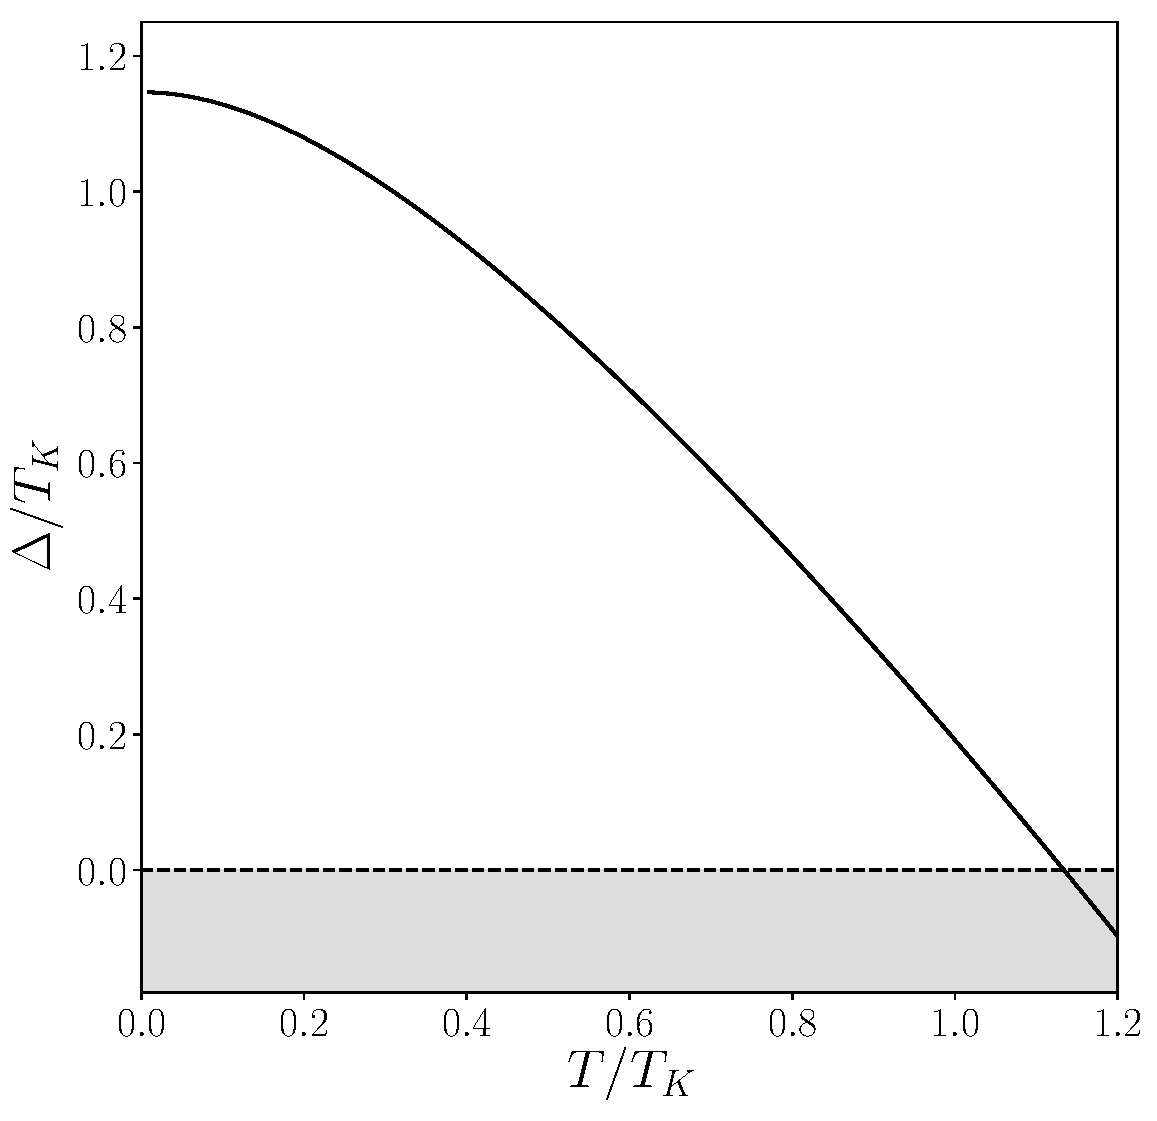
\includegraphics[width=0.7\textwidth]{Figures/delta_vs_T.pdf}
\caption{A plot of the order parameter $ \Delta $ against the temperature $ T $, with both axes normalised by the Kondo temperature $ T_K $. The shaded region below the $ \Delta = 0 $ line indicates a non-physical region of the order parameter. The phase transition occurs at $ T_c \approx 1.13 ~ T_K $.}
\label{fig:delta_vs_T}
\end{figure}

From this plot it may be seen that the first derivative of the order parameter, $ \frac{d \Delta}{d T} $, is discontinuous at $ T = T_c $ if intervening by not allowing $ \Delta $ to become negative. This has the consequence (see Appendix~\ref{sec:discontinuity}) that $ \frac{d^2 F}{d T^2} $ is also discontinuous, characteristic of a second-order phase transition as opposed to a crossover. (Section~\ref{subsec:manipulating_PT} will investigate whether judiciously choosing the temperature dependence of the original soft-constraint parameter $ K \rightarrow K(T) $ can remove this phase transition.)

% Should maybe include the actual derivative here also

% Go through the work you did in trying to see if a phase transition can be removed
% Show the plot of the order parameter
% Want to know if the extra Fermi function dependence of kappa is still captured by K being a function of temperature

\subsection{Limitations of a Constant Soft-Constraint Parameter}

Before starting to artificially influence the temperature dependence of the model by promoting $ K \rightarrow K(T) $, one might question whether or not this is a natural thing to do in the first place. In solving the mean-field equations as we did in Section~\ref{subsec:solving_MF}, we absorbed the analytically difficult $ \langle h^{\dagger} h \rangle $ term into a free parameter $ \kappa $ that allowed us to reduce the mean-field equations to a single equation, namely Eq~\eqref{eq:soln_delta}. This strategy, however, came at the cost of expressing $ \Delta $ in terms of $ \kappa $ and \emph{not} the elementary parameter $ K $ which originally appeared in the introduction to the soft-constraint approach. We shall now observe the behaviour that would arise if insisting that $ K $ were instead held \emph{constant}.

Keeping the mean-field equations in terms of $ K $ and $ T $, we are left to solve two simultaneous equations involving $ \lambda_{SC} $ and $ \Delta $:
\begin{equation}
\psi \left( \frac{1}{2} + \frac{z^2 \Delta}{2 \pi T} \right) = \ln{\frac{T_K}{T}} - \ln{\left( 2 \pi \sqrt{\rho J} \right)} + \frac{1}{\rho J} \left[ 1 - \frac{1}{z^2} \right] ~ ,
\end{equation}

\begin{equation}
\quad \lambda_{\text{SC}} = \frac{8}{\pi \rho J} \frac{\Delta}{z^2} \left( 1 - \frac{2 K}{1 + e^{- \beta K \lambda_{\text{SC}}}} \right) ~ ,
\end{equation}

where $ z^2 = 4 K \left( 1 - K / (1 + e^{- \beta K \lambda_{\text{SC}}}) \right) / \left({1 + e^{- \beta K \lambda_{\text{SC}}}} \right) $. It may be appreciated that simply rearranging these equations for $ \Delta $ is now made impossible.

Nevertheless, it is still possible to make some progress by parameterising the above equations in terms of $ s \equiv \beta \lambda_{\text{SC}} $, and plotting the quantities $ \Delta / T_K $ and $ T / T_K $ along both axes according to:
\begin{equation}
\left( \frac{T}{T_K} \right) = \frac{1}{2 \pi \sqrt{\rho J}} ~ e^{(1 - z^{-2}) / (\rho J)} ~ \exp{\left[- \psi \left( \frac{1}{2} + \frac{\rho J ~ z^4 ~ s}{16 (1 - 2 K / (1 + e^{- K s}))} \right) \right]} ~ ,
\label{eq:parametric_T}
\end{equation}

\begin{equation}
\left( \frac{\Delta}{T_K} \right) = \frac{\pi \rho J ~ z^2}{8 (1 - 2 K / (1 + e^{- K s}))} \left( \frac{T}{T_K} \right) s ~ .
\label{eq:parametric_delta}
\end{equation}

\begin{figure}[ht]
\centering
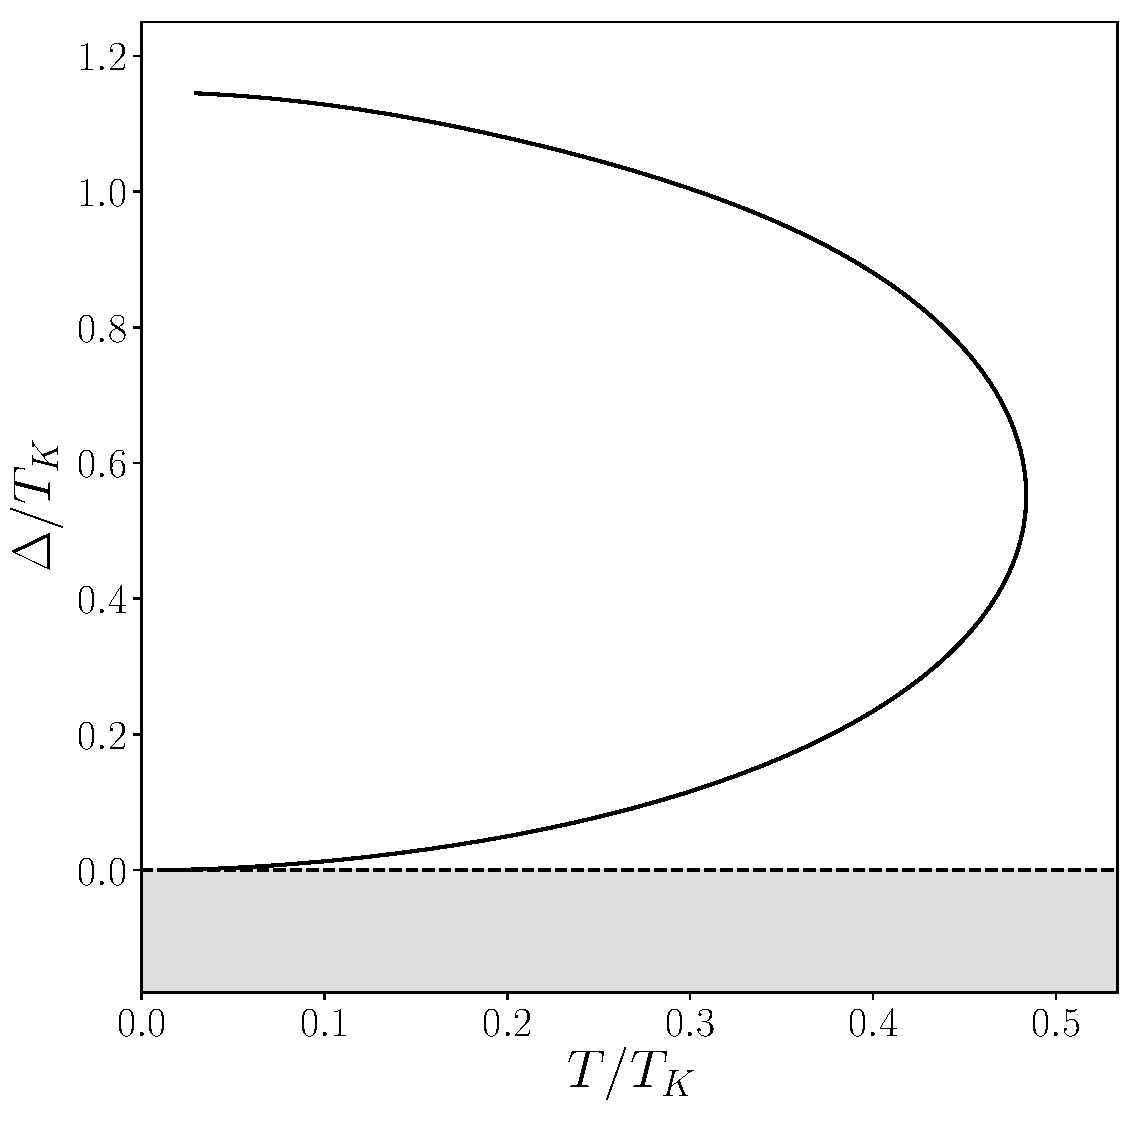
\includegraphics[width=0.7\textwidth]{Figures/new_delta_vs_T_parametric.pdf}
\caption{A plot of the order parameter $ \Delta $ against the temperature $ T $, produced parametrically for the case of constant $ K $. The one-to-many mapping is not a physical function and so indicates a failure of the mean-field equations to pick out the minimal action.}
\label{fig:parametric}
\end{figure}

The resulting parametric plot, Figure~\ref{fig:parametric}, has a catastrophic shape in which there are no mean-field solutions beyond a certain temperature, but two extremal values of $ \Delta $ below this temperature.\footnote{This strange behaviour may look suspiciously like an artefact of the algebraic manipulations used to achieve the parametric form of Eq~\eqref{eq:parametric_T} and Eq~\eqref{eq:parametric_delta} (such as $ s $ not being an injective parameterisation), but this functional form is also reproduced when numerically solving the mean-field equations.} This suggests a breakdown of the mean-field equations and from this clearly unphysical behaviour we conclude that $ K $ must indeed have some temperature dependence if it is to accurately describe any finite temperature features of the model at all.

\subsection{Manipulating the Nature of the Phase Transition}
\label{subsec:manipulating_PT}

We have seen that neither constant $ K $ nor $ \kappa $ can reproduce a crossover from a strongly-coupled to weakly-coupled phase at finite temperature. We now investigate whether a suitable choice of $ \kappa \rightarrow \kappa(T) $ can remove this second-order phase-transition.

The first question to ask is whether it is possible for mean-field $ \Delta $ to only \emph{asymptotically} approach the weakly-coupled phase as temperature is increased, thereby not assuming a piecewise form. Consider choosing a different value for the soft-constraint parameter $ \widetilde{\kappa} $ such that $ z^2 \rightarrow \widetilde{z^2} = \alpha z^2 $. To see whether the form of $ \Delta(T) $ will change significantly upon making this choice, one can look at the new mean-field equation for $ \Delta $:
\begin{equation}
\psi \left( \frac{1}{2} + \frac{\alpha z^2 \Delta}{2 \pi T} \right) = \ln{\frac{D}{2 \pi T}} - \frac{1}{J \rho ~ \alpha z^2} ~ .
\end{equation}
When rescaling axes according to
\begin{equation}
\widetilde{T} = T \cdot e^{- \left( \frac{1}{\alpha} - 1 \right) / (J \rho z^2)} ~, \quad \widetilde{\Delta} = \Delta \cdot \alpha e^{- \left( \frac{1}{\alpha} - 1 \right) / (J \rho z^2)} ~ ,
\end{equation}
this equation reduces to nothing more than the original mean-field equation of Eq~\eqref{eq:soln_delta}, only this time in terms of $ \widetilde{\Delta} $ and $ \widetilde{T} $.
Therefore, choosing a different constant value of $ \kappa $ cannot change the shape of $ \Delta(T) $. Consequently, even if we promote $ \kappa \rightarrow \kappa(T) $ \footnote{After all, any temperature-dependent $ \kappa(T) $ is just switching between different `constant $ \kappa $' curves.}, the above mean-field condition will have an unavoidable $ \Delta = 0 $ solution at some finite temperature below
\begin{equation}
T^{\star}_c = T_K \cdot e^{- \psi \left( \frac{1}{2} \right)} / \left( 2 \pi \sqrt{\rho J} \right)~.
\end{equation}

Another option is to attempt to match successive derivatives of $ \Delta $ at the transition such that $ F $ will be continuous in all its derivatives. Trying to match all derivatives of a piecewise function that is analytic on both sides is conceptually dubious, however. This can be argued by saying that if all successive derivatives \textit{were} chosen to match, then both sides would share a Taylor series expansion about that point and hence be described by the same function, without need for a piecewise definition. Unless resorting to non-analytic functions, increasing the order of the phase transition is the closest one could get to a crossover.\footnote{Empirically, all derivatives of $ \Delta $ can be made to vanish by choosing $ \frac{1}{J \rho z^2} = \frac{1}{J \rho z_0^2} - \ln{\frac{T}{T_c}} $, but this forces $ \Delta = 0 $ at all temperatures (clearly undesirable) and contradicts the existing limits on the magnitude of $ \kappa $.}

With this in mind, we shall see what can nevertheless be achieved by choosing the form of $ \kappa (T) $. For example, let $ \kappa_0 $ be the value of the soft-constraint parameter that correctly picks out the Kondo temperature as before.\footnote{$ \kappa_0 = \frac{1}{2} \left( 1 - \sqrt{- \frac{1}{2} \rho J \ln{\rho J}} \right) $} Constructing $ \kappa(T) $ as
\begin{equation}
\kappa(T) = \kappa_0 + \delta \cdot \left[ \sech{\left( \frac{T}{t_1} \right)} + \tanh{\left( \frac{T - T_c}{t_2} \right)} \right] ~,
\end{equation}
can allow the order parameter to more gradually approach $ \Delta = 0$, as shown in Figure~\ref{fig:delta_smooth}, provided that $ t_1 $, $ t_2 $ and $ \delta $ are suitably chosen. The choice of the hyperbolic tangent above is somewhat arbitrary, but illustrates the principle that switching between $ (\kappa_0 - \delta) $ and $ (\kappa_0 + \delta) $ near the transition temperature can reduce the gradient to zero at the transition. (The hyperbolic secant term, on the other hand, serves to recover some of the zero-temperature behaviour.) There likely exist other, better choices for $ \kappa(T) $, depending on the desired functional form of $ \Delta(T) $; the only requirement is that $ \frac{d \Delta}{d T} \rightarrow 0 $ as $ \Delta \rightarrow 0 $, which can be achieved by tuning the parameters of the function such that 
\begin{equation}
\frac{d \kappa}{d T} \Bigr|_{T = T_c} = \frac{4 J \rho}{T_c} \frac{\kappa^2_0 (1 - \kappa_0)^2}{(1 - 2 \kappa_0)} \quad \text{and} \quad \kappa(T_c) = \kappa_0 ~ .
\end{equation}

\begin{figure}
\centering
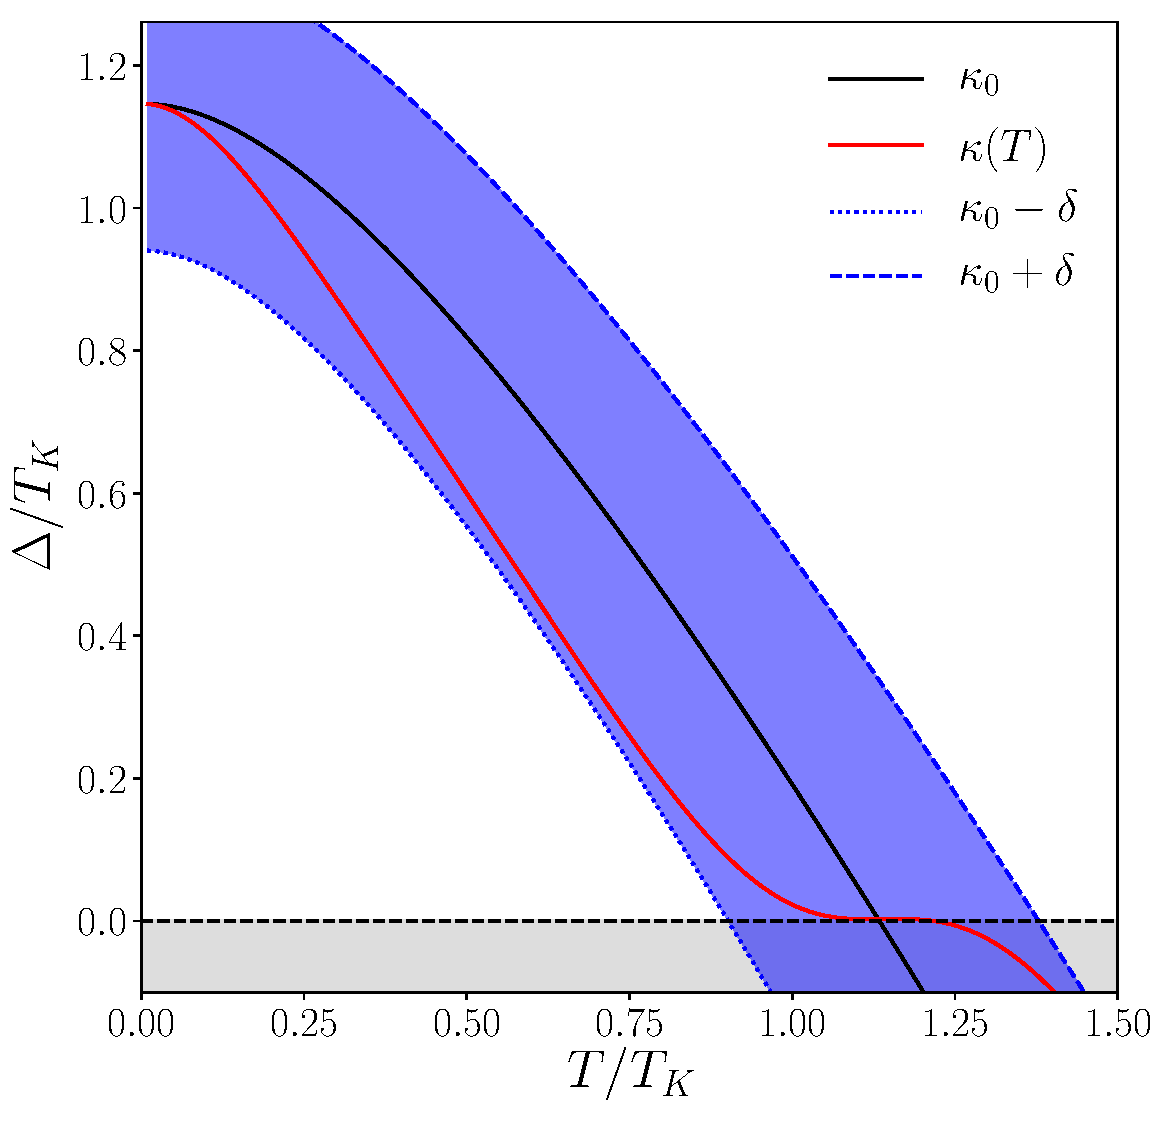
\includegraphics[width=0.7\textwidth]{Figures/range_delta_vs_T.pdf}
\caption{A plot where the form of $ \kappa(T) $ is chosen to increase the order of the transition. Here, $ \kappa(T) $ is given by Eq~\eqref{eq:kappa_temp} (with $ \delta \approx 0.018 $, $ t_1 \approx \frac{1}{5} T_K $ and $ t_2 \approx \frac{4}{17} T_K $ for $ \rho J = 0.16 $) and switches from one constant $ \kappa $ curve to another. This allows the order parameter to take on any shape bounded by the blue shaded region, whose width is determined by the magnitude of $ \delta $.}
\label{fig:delta_smooth}
\end{figure}

One glaring deficiency of this analysis is that it is still unclear how $ K(T) $ should be chosen in the first place, since it would in general require solving
\begin{equation}
\kappa(T) = \frac{K(T)}{1 + e^{- \beta \lambda_{\text{SC}} K(T)}} ~ ,
\label{eq:kappa_temp}
\end{equation}
for which the simple relation $ K(T) \approx 2 \kappa(T) $ only holds near $ T \approx T_c $. \footnote{For what it's worth, a solution can be approached through the infinite expression
\begin{equation}
K = \kappa  \left( 1 + \exp{\left( - \beta \lambda_{\text{SC}} \kappa \left( 1 + \exp{\left( - \beta \lambda_{\text{SC}} \kappa \left( 1 + \ldots \right) \right)} \right) \right)} \right).
\end{equation}}

% Want to say that maybe the PT can be removed?